\documentclass{article}
\usepackage{a4wide}
\usepackage[english]{babel}
\usepackage{amsmath}
\usepackage{amssymb}
\usepackage{dsfont}
%\usepackage[dvips]{epsfig}
%\usepackage{graphicx}
\usepackage{fancyhdr}
\usepackage{listings}
\usepackage{nomencl}
\usepackage[pdftex]{graphicx}

\pagestyle{fancy}
\lhead{\footnotesize \parbox{11cm}{A.J. H\"ormer, E. Vontobel, A. Novacek}}
\rhead{\footnotesize {Plexos Project}}
\chead{\footnotesize {TET4135}}

\title{Report Plexos Project}
\author{Andreas Johann H\"ormer, Eva Vontobel, Adam Novacek}
\date{\today}

\begin{document}
\thispagestyle{empty}
\maketitle
\thispagestyle{empty}
%\\[5cm]
\begin{center}
TET4135 Energiplanlegging\\[3cm]
Lab group:
\begin{itemize}
\item Andreas Johann H\"ormer
\item Eva Vontobel
\item Adam Novacek\\[3cm]
\end{itemize}
Report delivered: \\[6cm]
FACULTY OF INFORMATION TECHNOLOGY, MATHEMATICS AND ELECTRICAL ENGINEERING\\
NORWEGIAN UNIVERSITY OF SCIENCE AND TECHNOLOGY
\end{center}
\thispagestyle{empty}
\newpage
\tableofcontents
\thispagestyle{empty}
\newpage
\section*{Abstract}
\thispagestyle{empty}

\newpage
\setcounter{page}{1}
\section{Introduction}

\section{Theory}
\subsection{Methods in present work}
\subsection{intermittent resource handling}
\subsection{reservoir hydro handling}
\subsection{region exchange}
\subsubsection{Advantages}
\subsubsection{Disadvantages}
%-------------------------------------------------------------------------------
% Investment initiatives
%-------------------------------------------------------------------------------
\subsection{investment initiatives for renewable sources}
\begin{itemize}
\item investment support\\
One time financial support to cover part of the investment costs.  The support is large enough to make the investment profitable. Some differences can be used for fine tuning, e.g. more support for wind power in areas with less wind.
\begin{itemize}
\item advantages
\begin{itemize}
\item possibility of finetuning
\end{itemize}
\item disadvantages
\begin{itemize}
\item requires much capital at beginning
\item no incentive to roduce
\item limited security for investor
\item in case of fine tuning: much administration
\end{itemize}
\end{itemize}
\item tendering\\
Auction for a certain amount of capacity which shall be installed. Won by the offers requiring the lowest support. This initiative is also done as investment support, but with a tendering procedure. Providers are asked for support bids, the cheapest one gets the support.
\begin{itemize}
\item advantages
\begin{itemize}
\item competition between suppliers, therefore lower costs than investment support
\end{itemize}
\item disadvantages
\begin{itemize}
\item same as investment support, but
\item less predictability
\item prone to corruption
\end{itemize}
\end{itemize}
\item feed-in tariff\\
A fixed price for feeded kWh is payed for a predefined period.
\begin{itemize}
\item advantages
\begin{itemize}
\item promotion of mid-term and long-term technologies
\item investment security for producer
\end{itemize}
\item disadvantages
\begin{itemize}
\item possible risk of technology overfunding
\end{itemize}
\end{itemize}
\item premium\\
Like feed-in tariff, but instead of a fixed price an additional amount per kWh is paid to the producer.
\begin{itemize}
\item advantages
\begin{itemize}
\item market based
\end{itemize}
\item disadvantages
\begin{itemize}
\item less certainty than feed-in tariff
\end{itemize}
\end{itemize}
\item green certificates
This is a nordic system for supporting renewables. Some amount of certified energy has to be bought from energy suppliers, otherwise they are penalized. The intention is to build as much renewables as possible in short time. From 2020 new renewables are not certified any more, so the possibility to get enough certified power decreases and the risk of getting penalized increases.
\begin{itemize}
\item advantages
\begin{itemize}
\item control of total amount of renewables
\item efficient market-based solution
\end{itemize}
\item disadvantages
\begin{itemize}
\item less certainty than feed-in
\item complex
\item high administration costs
\end{itemize}
\end{itemize}
\end{itemize}

\section{Analysis}

%-------------------------------------------------------------------------------
% MT Schedule
%-------------------------------------------------------------------------------
\subsection{MT Schedule}
The medium term schedule is done for one year. Three different scenarios (low, normal, high inflow) to the reservoirs in Norway and Sweden are simulated. The different scenarios are described below.

%-------------------------------------------------------------------------------
% normal inflow scenario
%-------------------------------------------------------------------------------
\subsubsection{normal inflow scenario}
For this case a normal inflow scenario was chosen. The inflow accords to the average inflow in a year in Norway and Sweden.
\paragraph{optimal generation dispatch\\}
The optimal generation dispatch for normal inflow for Germany can be seen in figure \ref{fig:MTgenerationGnormal}. The generation dispatch for swedish generation units can be seen in figure \ref{fig:MTgenerationSnormal}, the norwegian dispatch is shown in figure \ref{fig:MTgenerationNnormal}.
\begin{itemize}
\item Germany\\
The nuclear power plants as well as the small coal power plant are running the whole year with full capacity for serving the base load. It can be obtained that in the winter is less solar power produced than in the summer, but more wind power is generated. The oil and small/medium gas generation units are hardly producing any power.
\item Sweden\\
The base load in Sweden is fully covered by nuclear and coal power. In summer some peak load is generated with small hydro, in winter the peak load is mainly covered with reservoir hydro. No power is produced with oil power plants, only small amount with gas generation.
\item Norway\\
In Norway more or less all power is produced by hydro power. In winter the power generation is mainly done with reservoir hydro, in summer about half of the produced energy is done with small hydro power. Some additional power is produced with wind generation, the installed gas power plant is producing no energy.
\end{itemize}
\begin{figure}[htbp]
\begin{center}
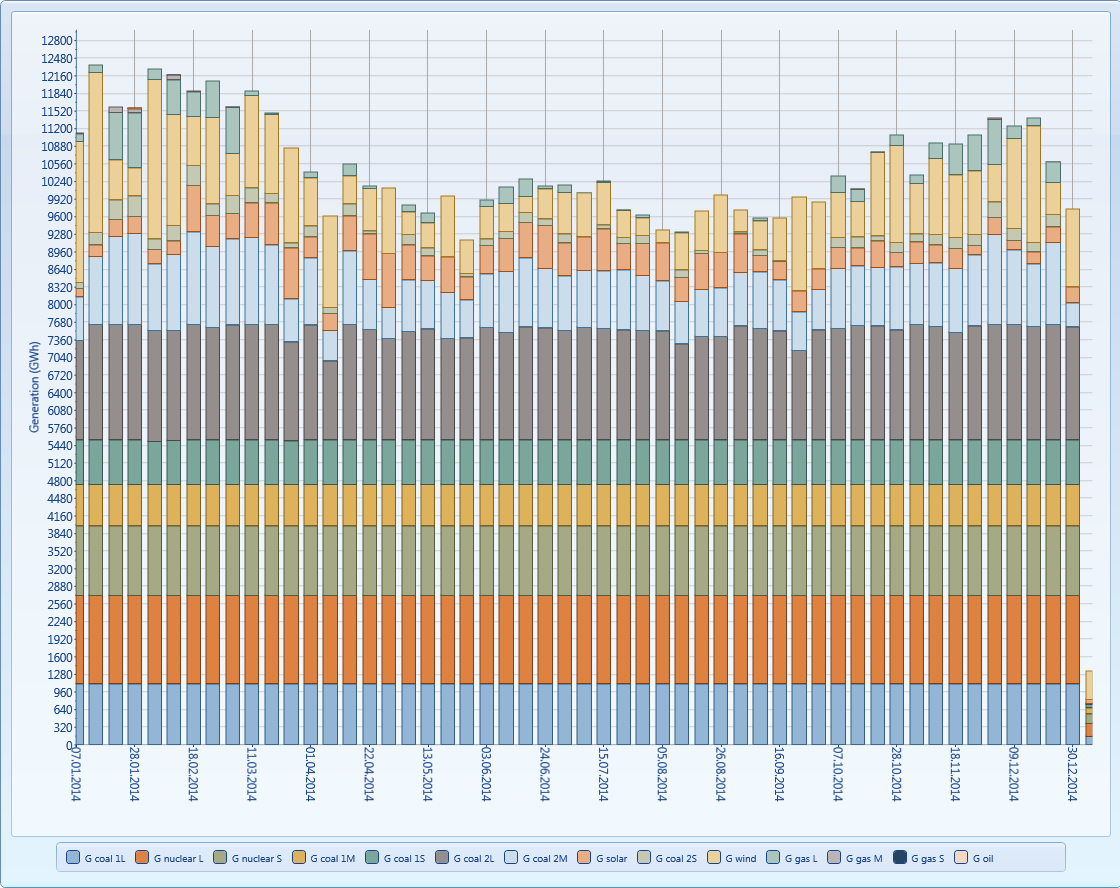
\includegraphics[width=13cm,keepaspectratio=true]{figures/MTgenerationG}
\caption{Optimal generation dispatch for Germany 2014 with normal inflow}
\label{fig:MTgenerationGnormal}
\end{center}
\end{figure}
\begin{figure}[htbp]
\begin{center}
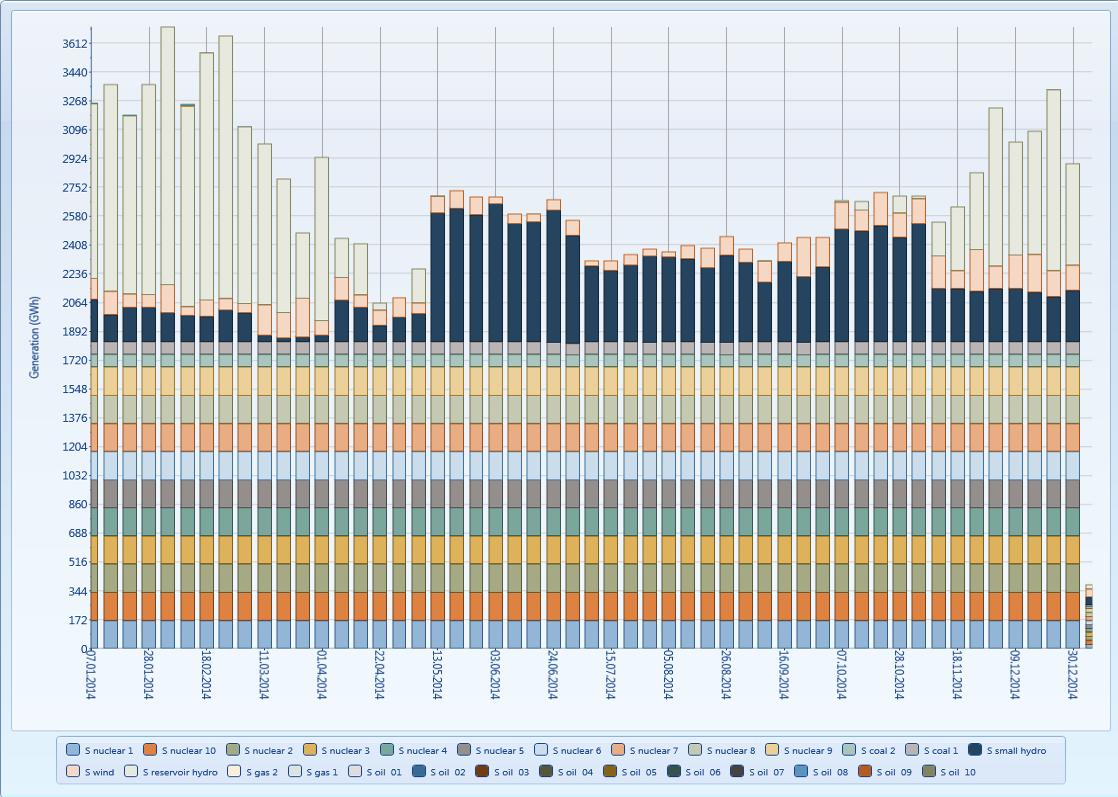
\includegraphics[width=13cm,keepaspectratio=true]{figures/MTgenerationS}
\caption{Optimal generation dispatch for Sweden 2014 with normal inflow}
\label{fig:MTgenerationSnormal}
\end{center}
\end{figure}
\begin{figure}[htbp]
\begin{center}
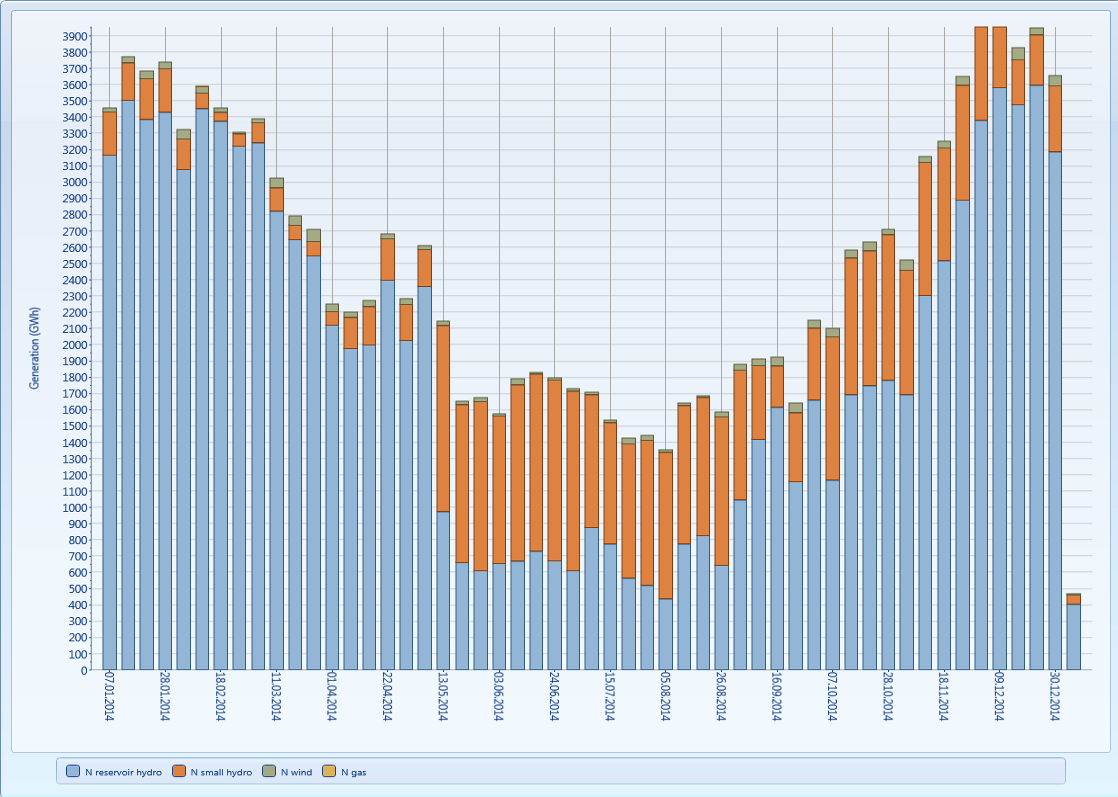
\includegraphics[width=13cm,keepaspectratio=true]{figures/MTgenerationN}
\caption{Optimal generation dispatch for Norway 2014 with normal inflow}
\label{fig:MTgenerationNnormal}
\end{center}
\end{figure}
\paragraph{transmission\\}
The transmission between the three countries Norway, Sweden and Germany is shown in figure \ref{fig:MTnodetransmissionnormal}. It is done not considering the flow direction, but the amount of power. Here it can be seen that most power flows between May and October. In winter there is very low flow between Norway and Sweden. The most continuous flow exists between Norway and Germany.
\begin{figure}[htbp]
\begin{center}
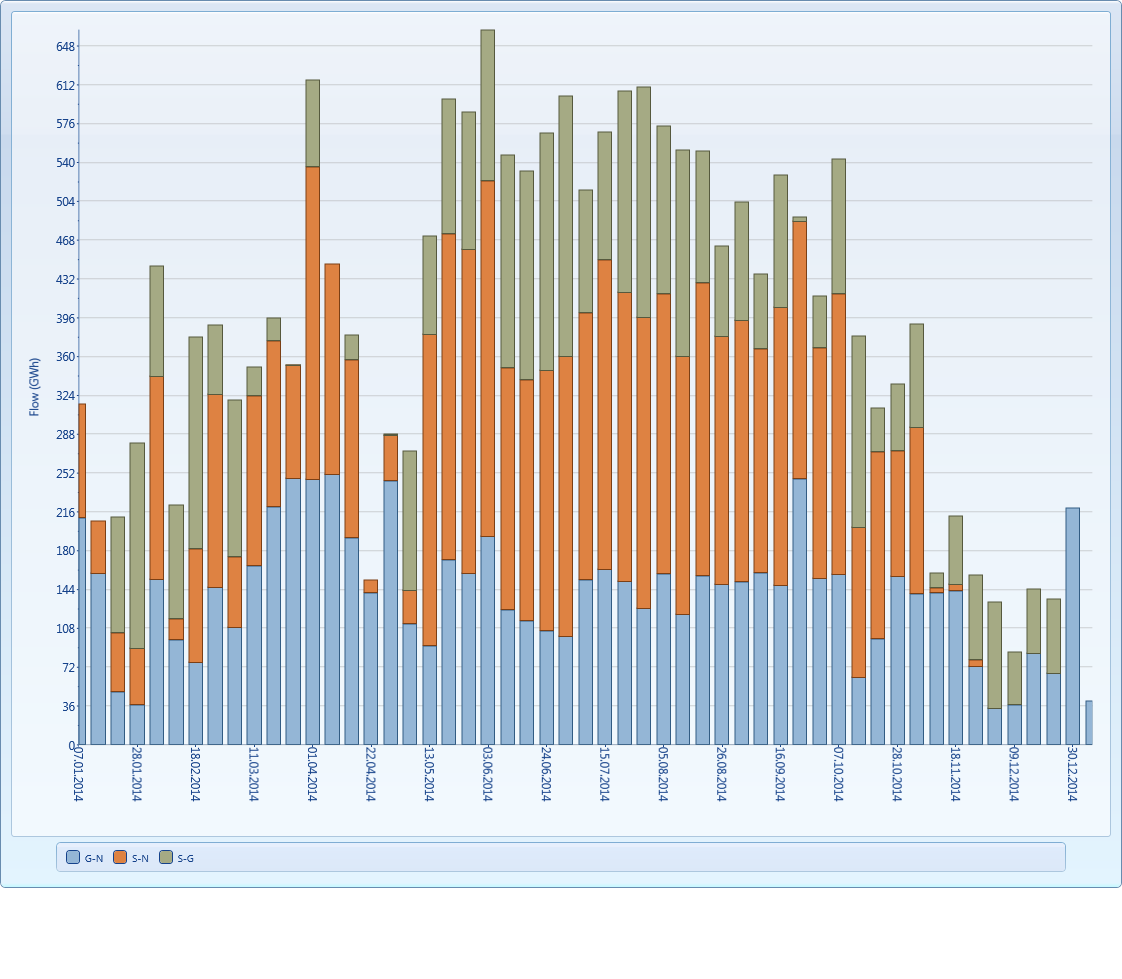
\includegraphics[width=13cm,keepaspectratio=true]{figures/MTnodetransmission}
\caption{Transmission between N/W/S with normal inflow}
\label{fig:MTnodetransmissionnormal}
\end{center}
\end{figure}
\paragraph{emission\\}
The total emissions for all countries together can be seen in figure \ref{fig:MTemissionsnormal}. The emissions can be interpreted in following way:
\begin{itemize}
\item Norway: Due to the fact that most power installed is done with renewables (hydro power, wind power) and only some small amount of gas power, there are hardly and $CO_2$-emissions in Norway.
\item Sweden: Some renewable energy and a large amount of nuclear power lead to small $CO_2$-emissions. 
\item Germany: The biggest amount of the produced emissions are emitted from german power plants. 
\end{itemize}
\begin{figure}[htbp]
\begin{center}
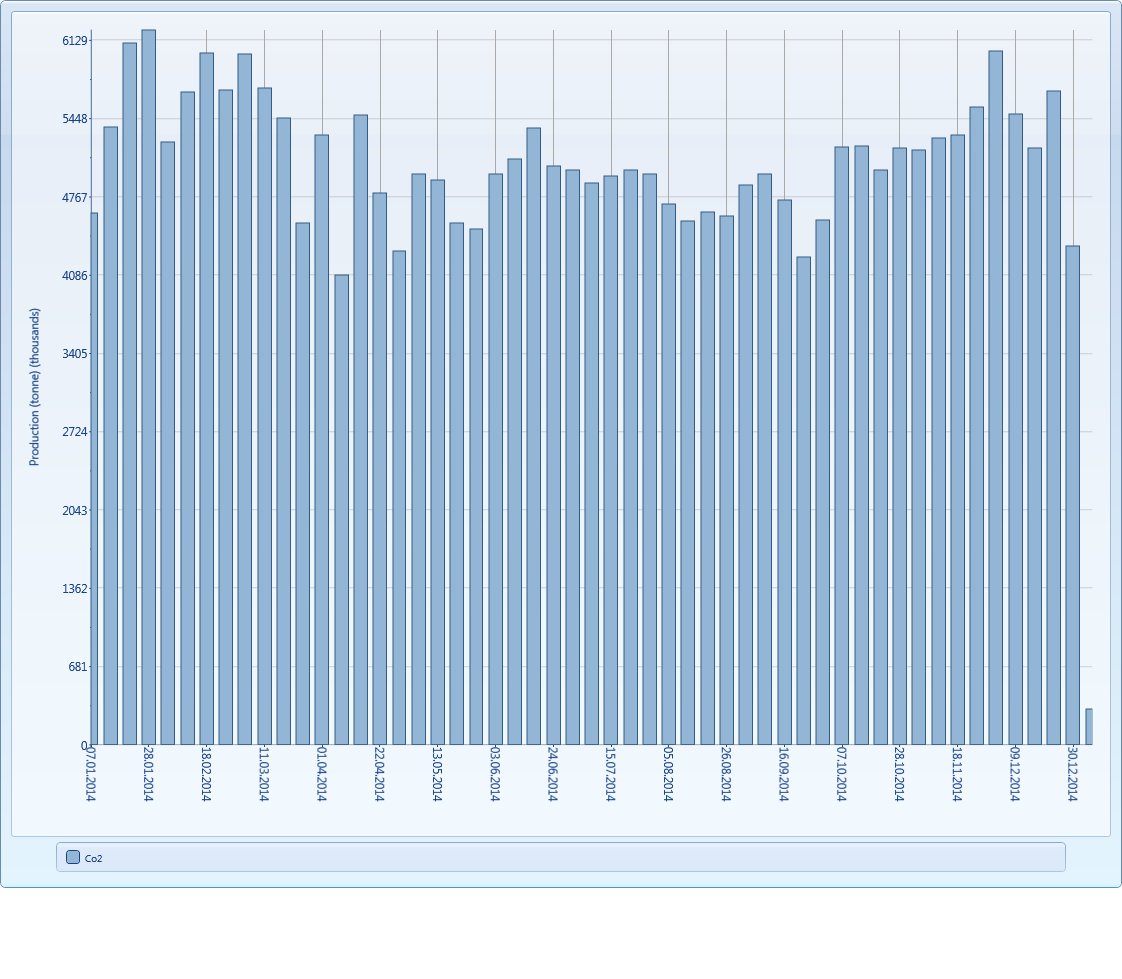
\includegraphics[width=13cm,keepaspectratio=true]{figures/MTCO2}
\caption{Total emissions for normal inflow 2014}
\label{fig:MTemissionsnormal}
\end{center}
\end{figure}
\paragraph{price\\}
Energy prices for the different weaks of 2014 for the analyzed countries are shown in figure \ref{fig:MTpricesnormal}. In this graph it can be obtained that prices in Norway are the lowest because of the high amount of renewable energy. The energy prices in Germany are the highest because of some coal and gas power. Generally the prices during the summer are lower than in the heating season. 
\begin{figure}[htbp]
\begin{center}
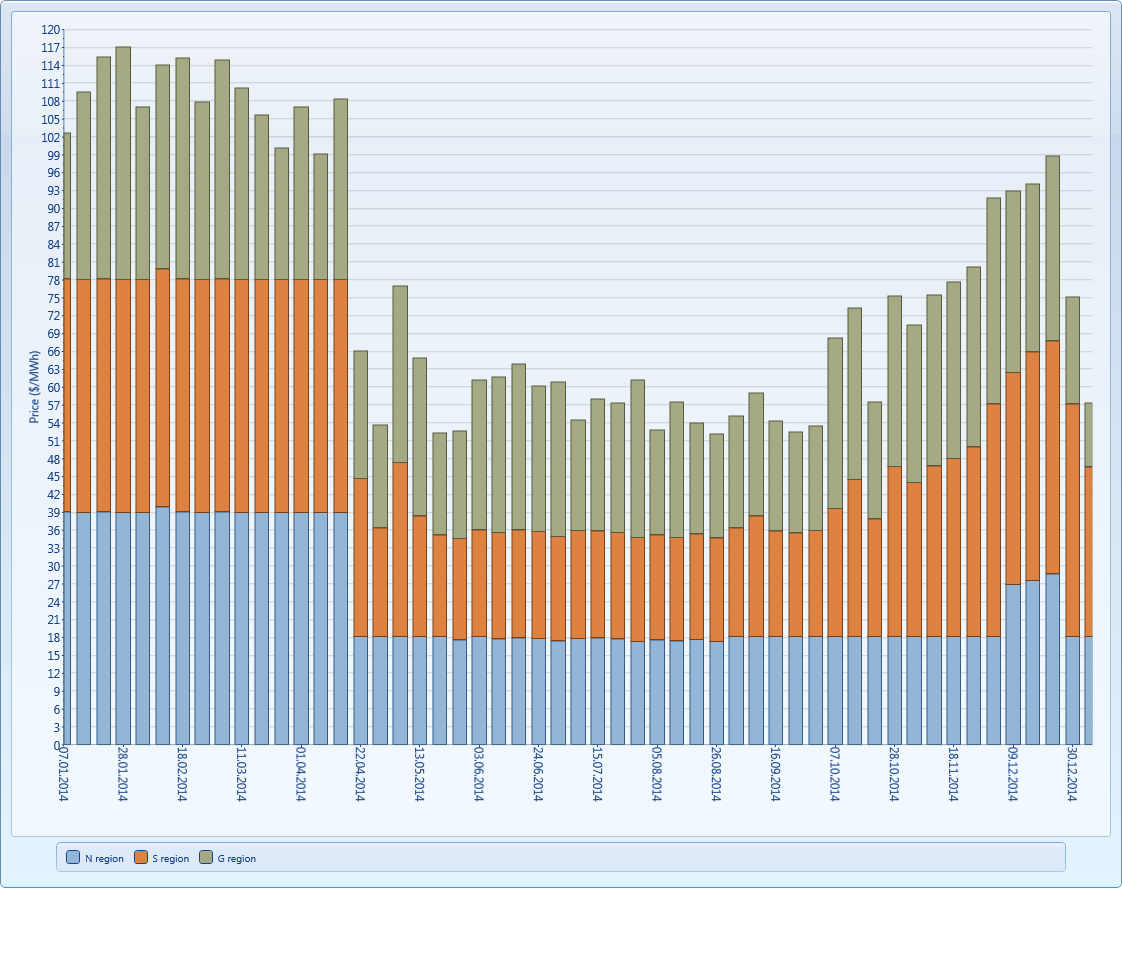
\includegraphics[width=13cm,keepaspectratio=true]{figures/MTprices}
\caption{Calculcated prices with normal inflow}
\label{fig:MTpricesnormal}
\end{center}
\end{figure}

%-------------------------------------------------------------------------------
% low inflow scenario
%-------------------------------------------------------------------------------
\subsubsection{low inflow scenario}
In this scenario a dry year with an inflow below the average was assumed. 
\paragraph{optimal generation dispatch\\}
The optimal generation dispatch is shown in figure \ref{fig:MTgenerationGdry} (Germany), figure \ref{fig:MTgenerationSdry} (Sweden) as well as figure \ref{fig:MTgenerationNdry} (Norway).
\begin{itemize}
\item Germany\\
Due to the fact that there is no renewable energy in Germany, the simulated results remain mostly the same. 
\item Sweden\\
Because of lower inflow the amount of energy produced with small hydro is lower than in average case. More energy is produced with reservoir hydro, but in dry years the production is a little bit lower than in the average simulation case.
\item Norway\\
Also in Norway the overall production decreases in the dry case. It can be obtained that during the heating season the difference to the average inflow is not significant. Most power is produced with reservoir hydro units. In summer the production is mainly done with small hydro power, which is quite different to the average. In dry years some gas production is used during the whole period.
\end{itemize}
\begin{figure}[htbp]
\begin{center}
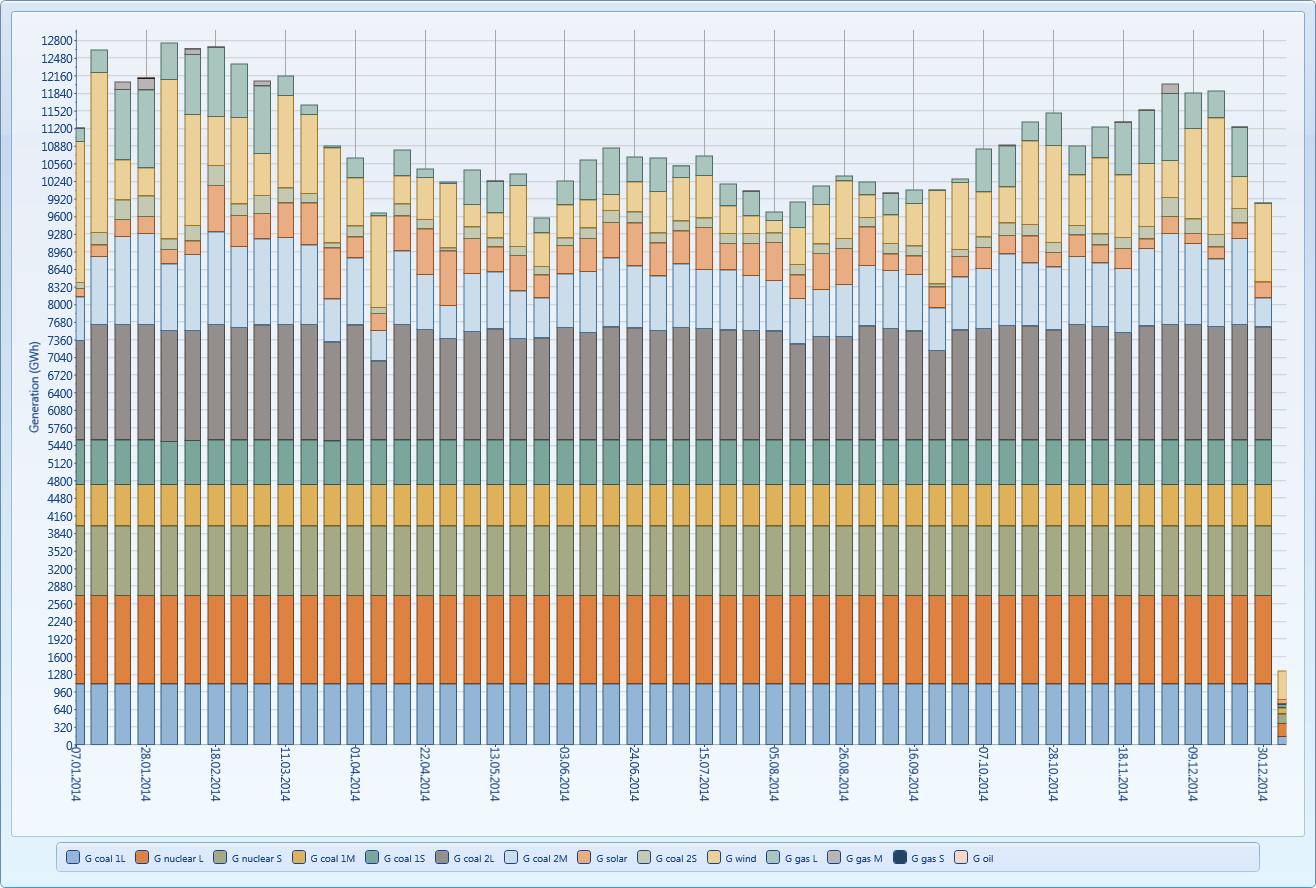
\includegraphics[width=13cm,keepaspectratio=true]{figures/drycase/MTgenerationGdry}
\caption{Optimal generation dispatch for Germany 2014 with low inflow}
\label{fig:MTgenerationGdry}
\end{center}
\end{figure}
\begin{figure}[htbp]
\begin{center}
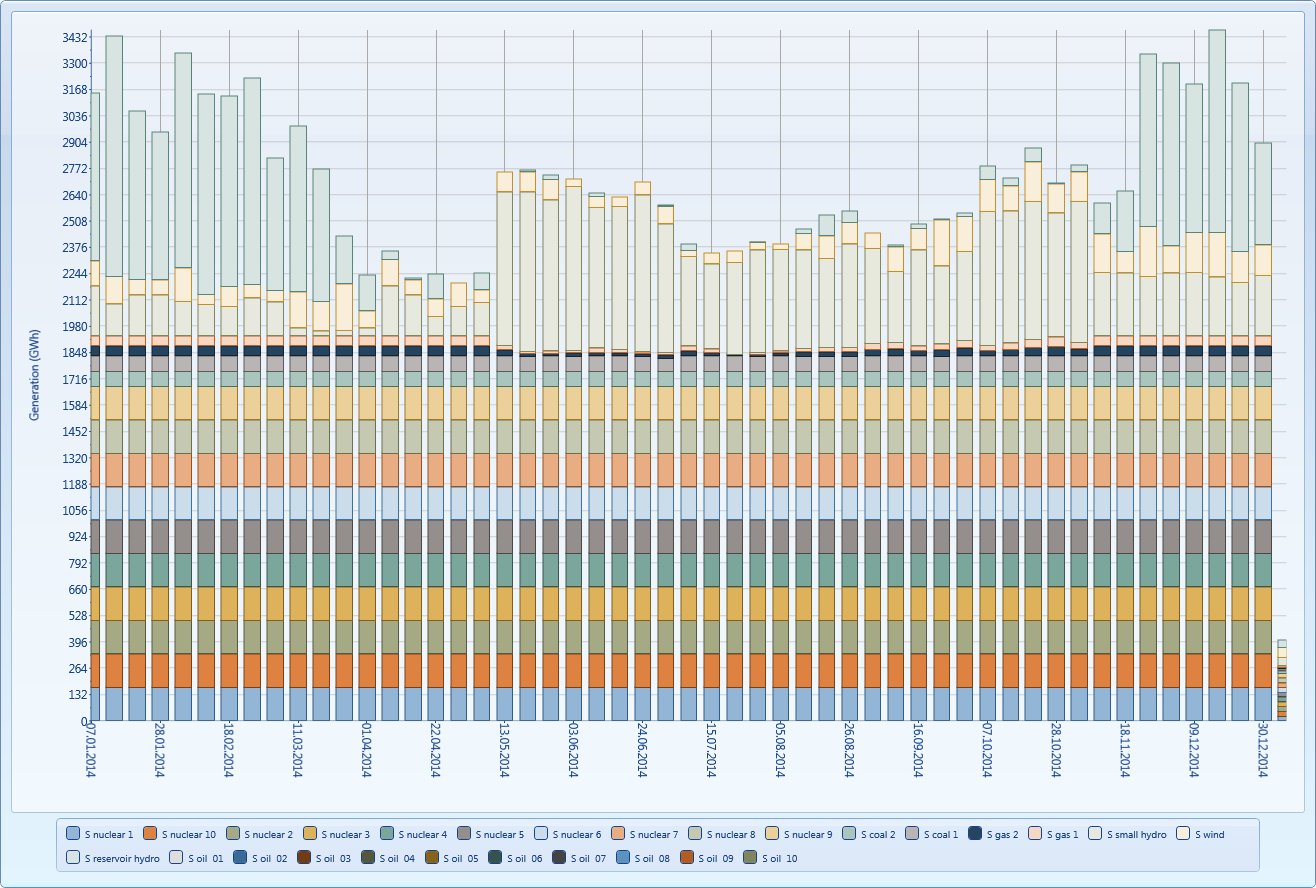
\includegraphics[width=13cm,keepaspectratio=true]{figures/drycase/MTgenerationSdry}
\caption{Optimal generation dispatch for Sweden 2014 with low inflow}
\label{fig:MTgenerationSdry}
\end{center}
\end{figure}
\begin{figure}[htbp]
\begin{center}
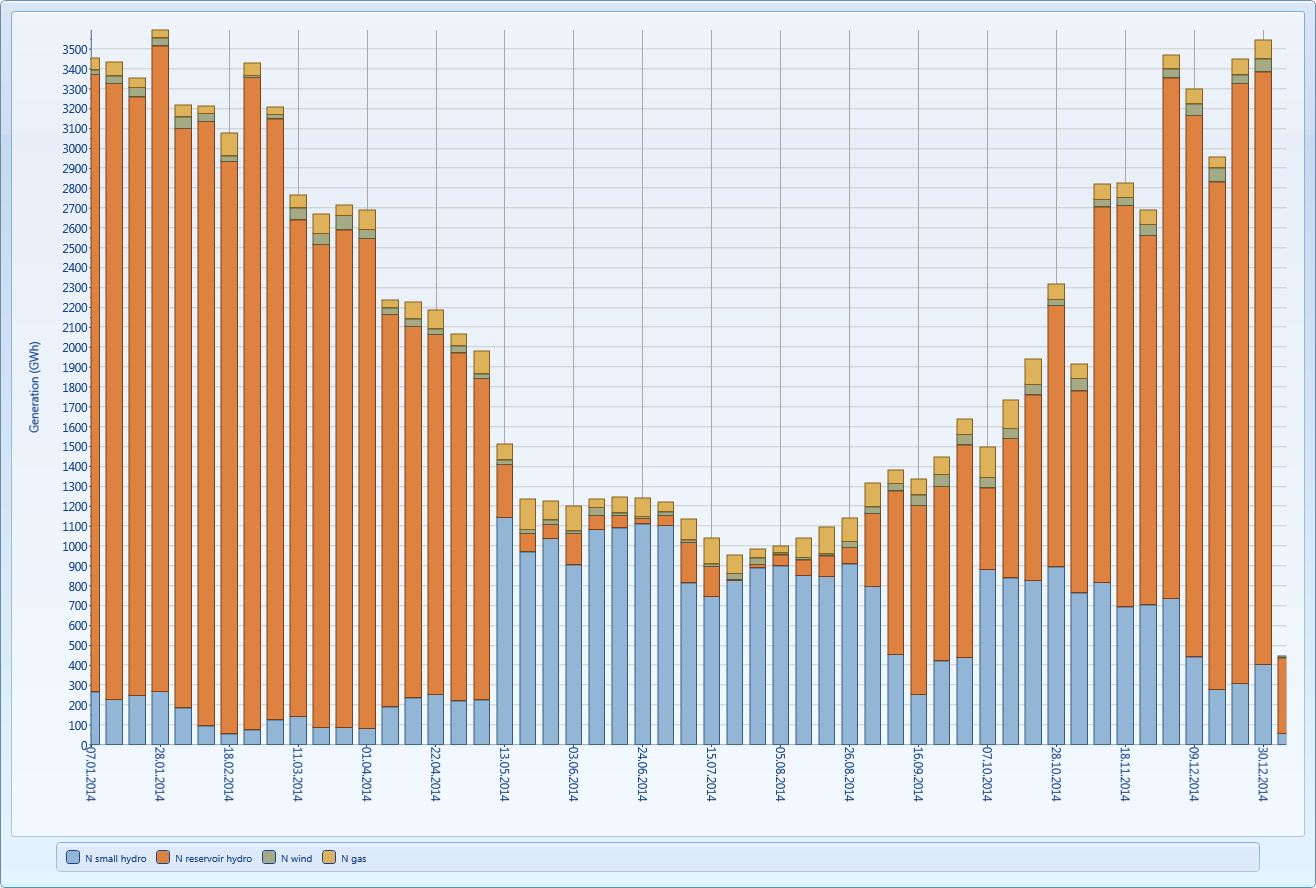
\includegraphics[width=13cm,keepaspectratio=true]{figures/drycase/MTgenerationNdry}
\caption{Optimal generation dispatch for Norway 2014 with low inflow}
\label{fig:MTgenerationNdry}
\end{center}
\end{figure}
\paragraph{transmission\\}
The power transmission on the powerlines between Norway, Sweden and Germany can be found in figure \ref{fig:MTnodetransmissiondry}. In the dry inflow case it can be seen that the flow between Germany and Norway is almost constant over the whole year. Between Sweden and Germany is hardly any flow, while the energy transmission in summer increases very much.
\begin{figure}[htbp]
\begin{center}
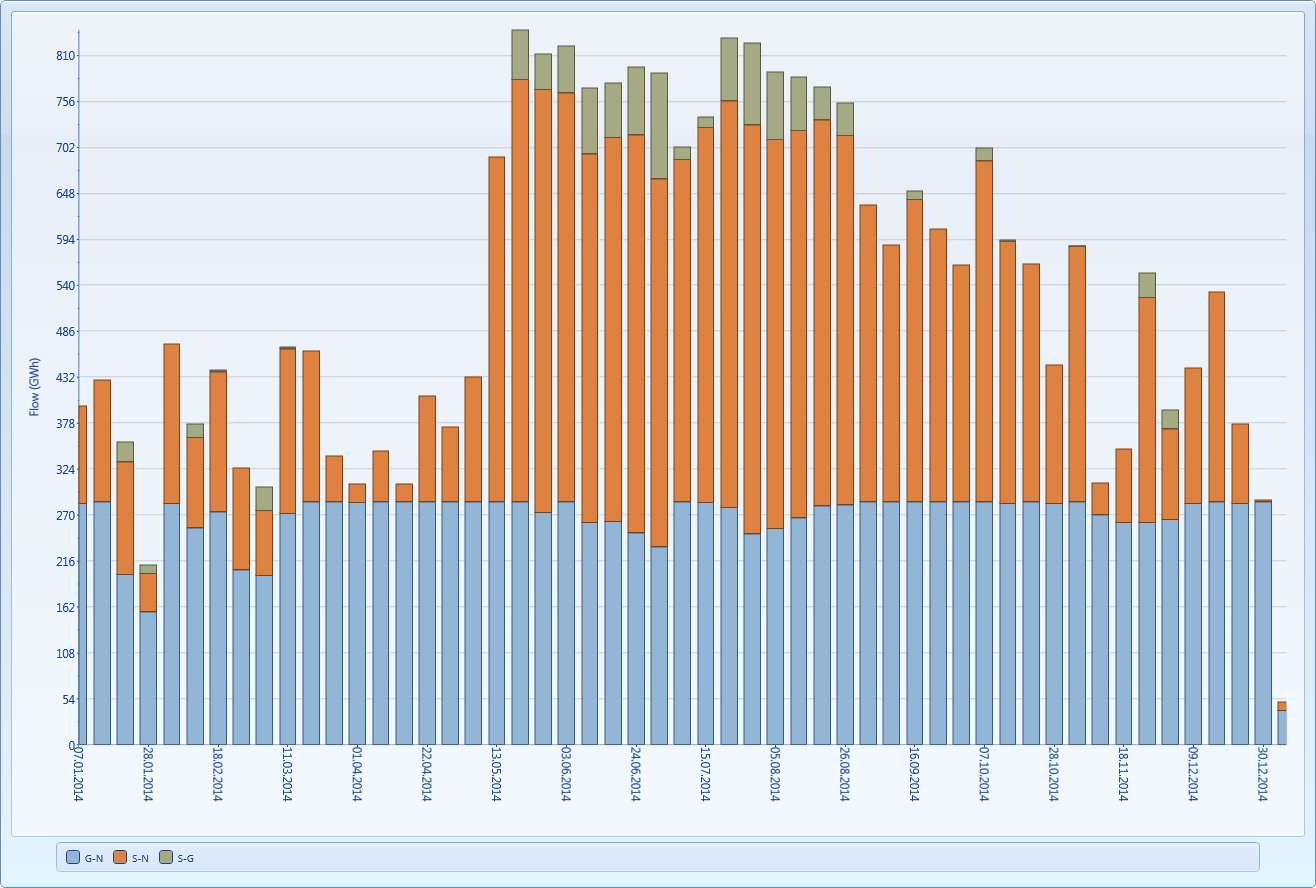
\includegraphics[width=13cm,keepaspectratio=true]{figures/drycase/MTnodetransmissiondry}
\caption{Transmission between N/W/S with low inflow}
\label{fig:MTnodetransmissiondry}
\end{center}
\end{figure}
\paragraph{emission\\}
$CO_2$-emissions for the whole year 2014 are shown in figure \ref{fig:MTemissionsdry}. Compared to the average inflow scenario the emissions in Norway are a little bit higher. This is because more power is produced with the gas generation unit. The most emissions are generated in Germany.
\begin{figure}[htbp]
\begin{center}
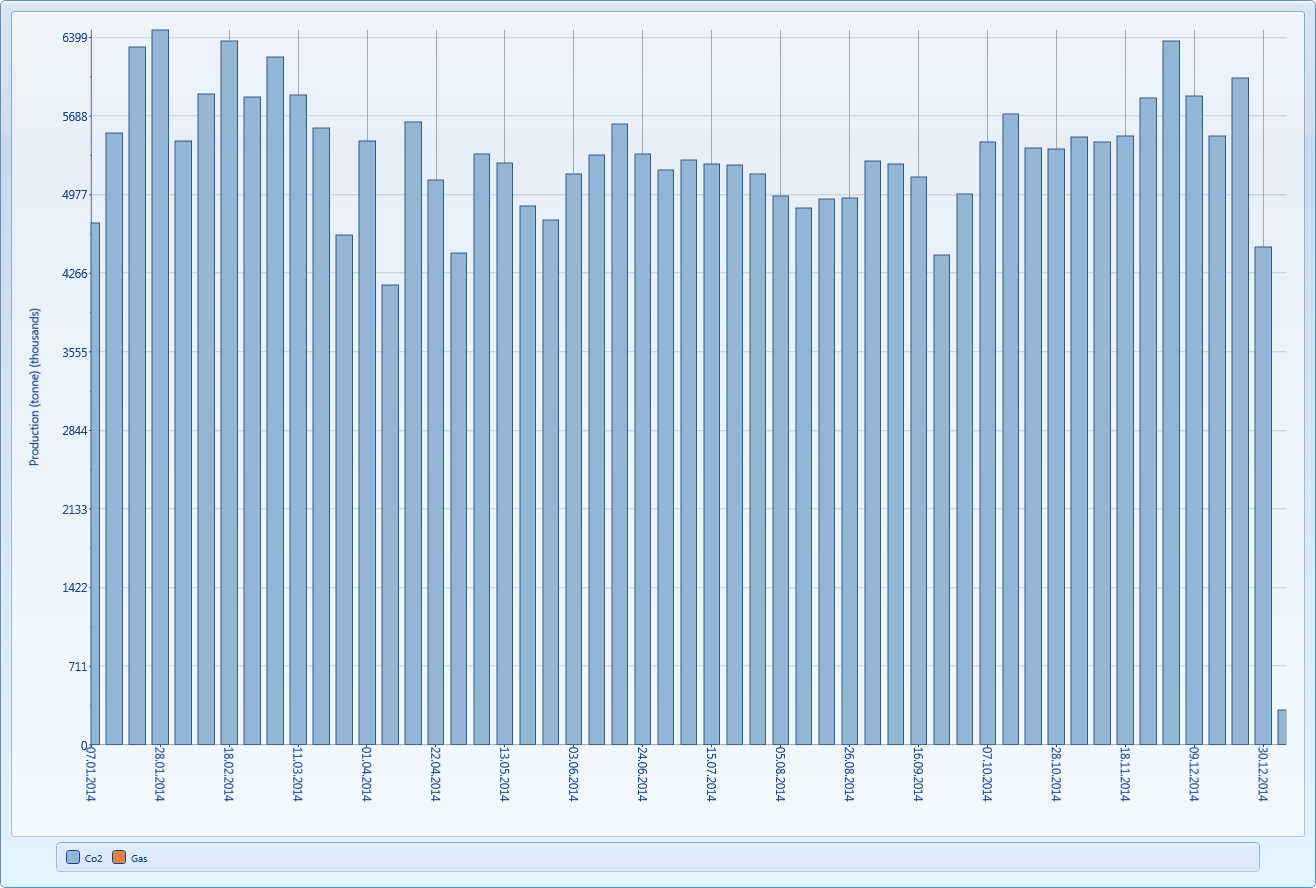
\includegraphics[width=13cm,keepaspectratio=true]{figures/drycase/MTCO2dry}
\caption{Total $CO_2$-emissions for low inflow 2014}
\label{fig:MTemissionsdry}
\end{center}
\end{figure}
\paragraph{price\\}
The energy prices for a dry year 2014 are plotted in figure \ref{fig:MTpriceslow}. Compared to the average inflow simulation, the prices are more constant over the year. The price level is higher due to lower renewable power production.
\begin{figure}[htbp]
\begin{center}
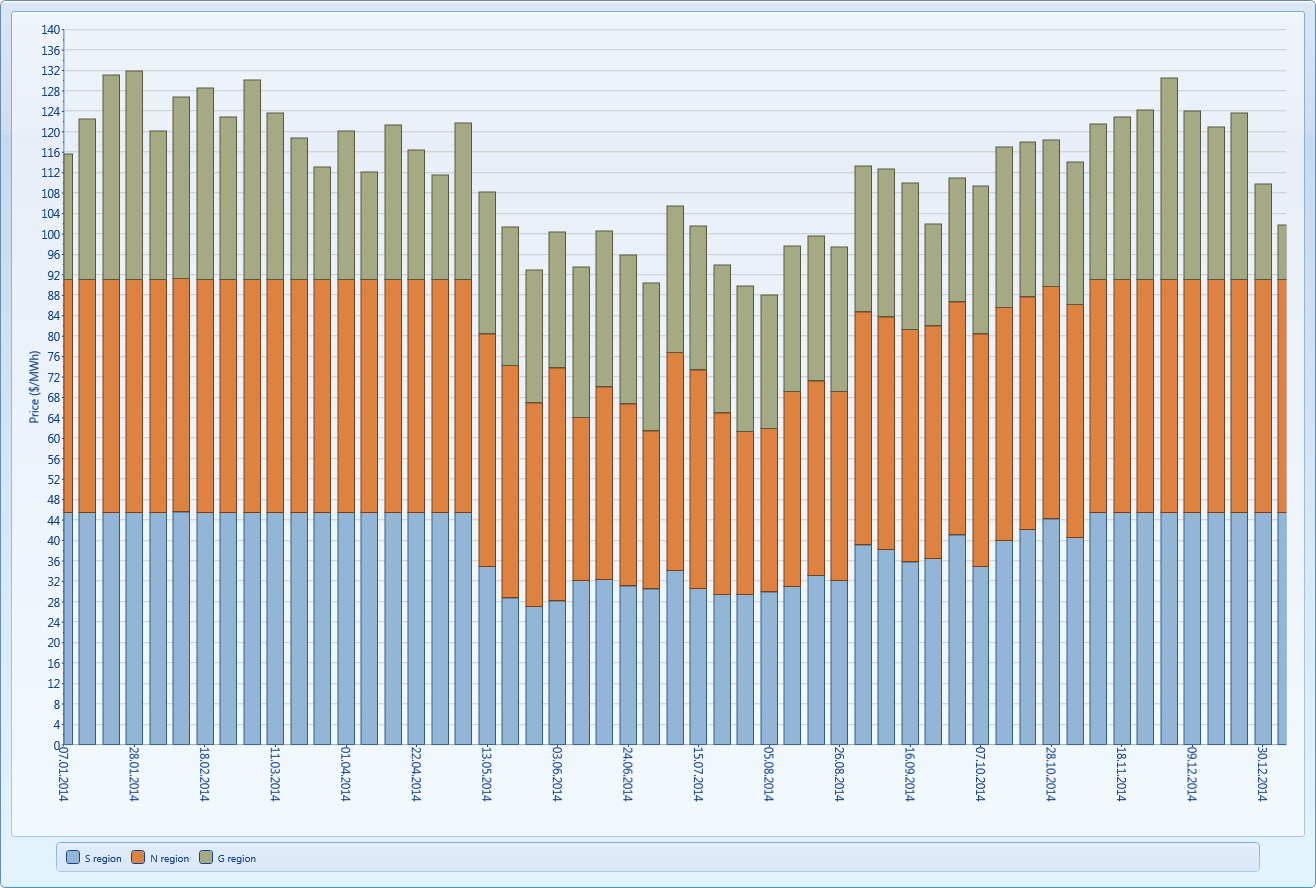
\includegraphics[width=13cm,keepaspectratio=true]{figures/drycase/MTpricesdry}
\caption{Calculcated prices with low inflow}
\label{fig:MTpriceslow}
\end{center}
\end{figure}

%-------------------------------------------------------------------------------
% high inflow scenario
%-------------------------------------------------------------------------------
\subsubsection{high inflow scenario}
This scenario uses a very wet year 2014. 
\paragraph{optimal generation dispatch\\}
Optimal generation for Sweden is shown in figure \ref{fig:MTgenerationSwet}. The generation dispatch for Norway can be seen in figure \ref{fig:MTgenerationNwet}, the german production in figure \ref{fig:MTgenerationGwet}.
\begin{itemize}
\item Germany\\
As in the average in the average inflow scenario and the low inflow scenario, the generation dispatch in Germany does not change significant due to the fact that no renewable power is installed.
\item Sweden\\
With high inflow the base load is also covered with nuclear and coal power. It can be obtained that mostly all peak power is produced with renewable generation units. During the heating season the peak power is produced with reservoir hydro power, in summer most peak power is produced with small hydro generation. Some additional power is produced with wind power during whole year, oil and gas generation is hardly used.
\item Norway\\
All power is produced by renewables in the high inflow scenario. The generation dispatch is like the dispatch in the average scenario, but more power is produced.
\end{itemize}
\begin{figure}[htbp]
\begin{center}
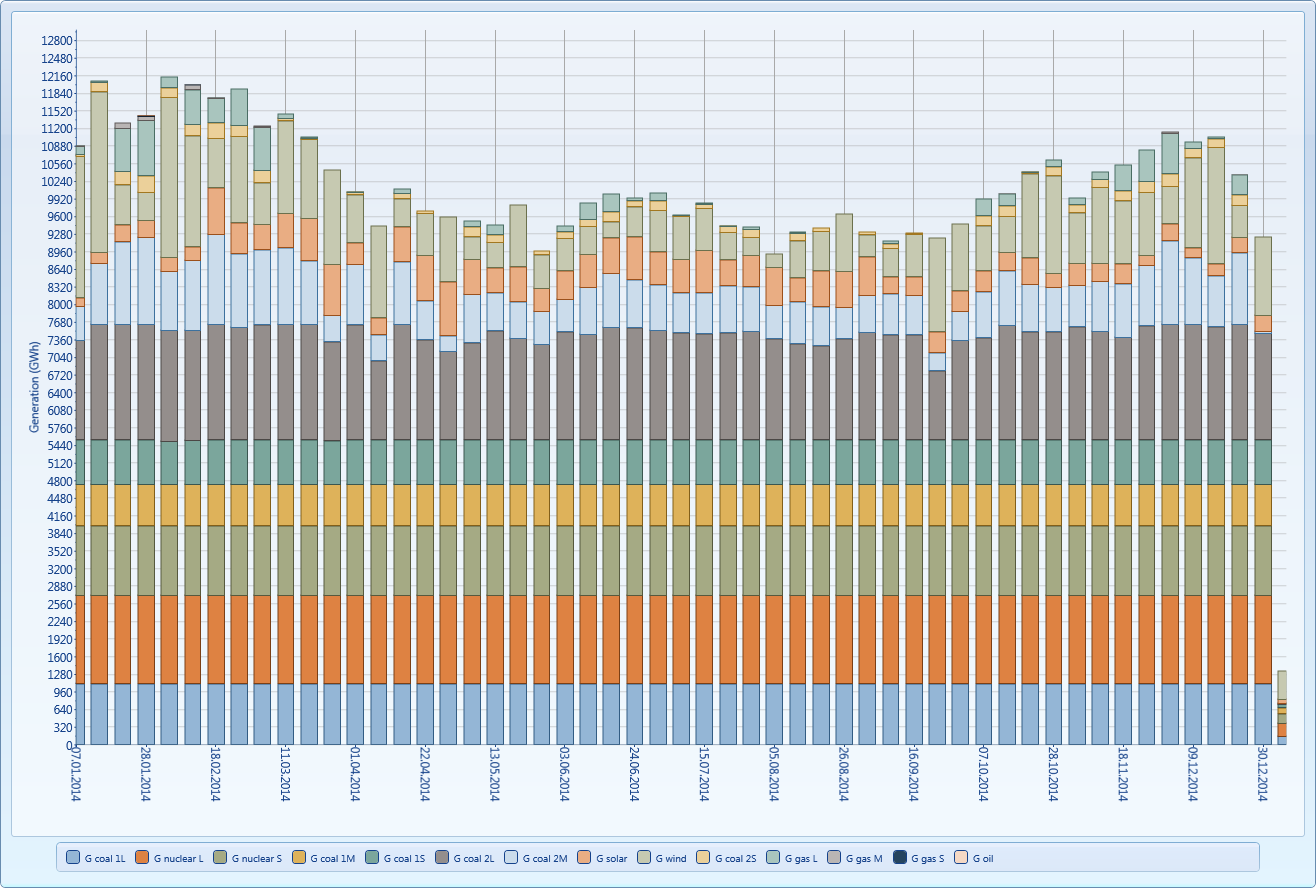
\includegraphics[width=13cm,keepaspectratio=true]{figures/wetcase/MTgenerationGwet}
\caption{Optimal generation dispatch for Germany 2014 with high inflow}
\label{fig:MTgenerationGwet}
\end{center}
\end{figure}
\begin{figure}[htbp]
\begin{center}
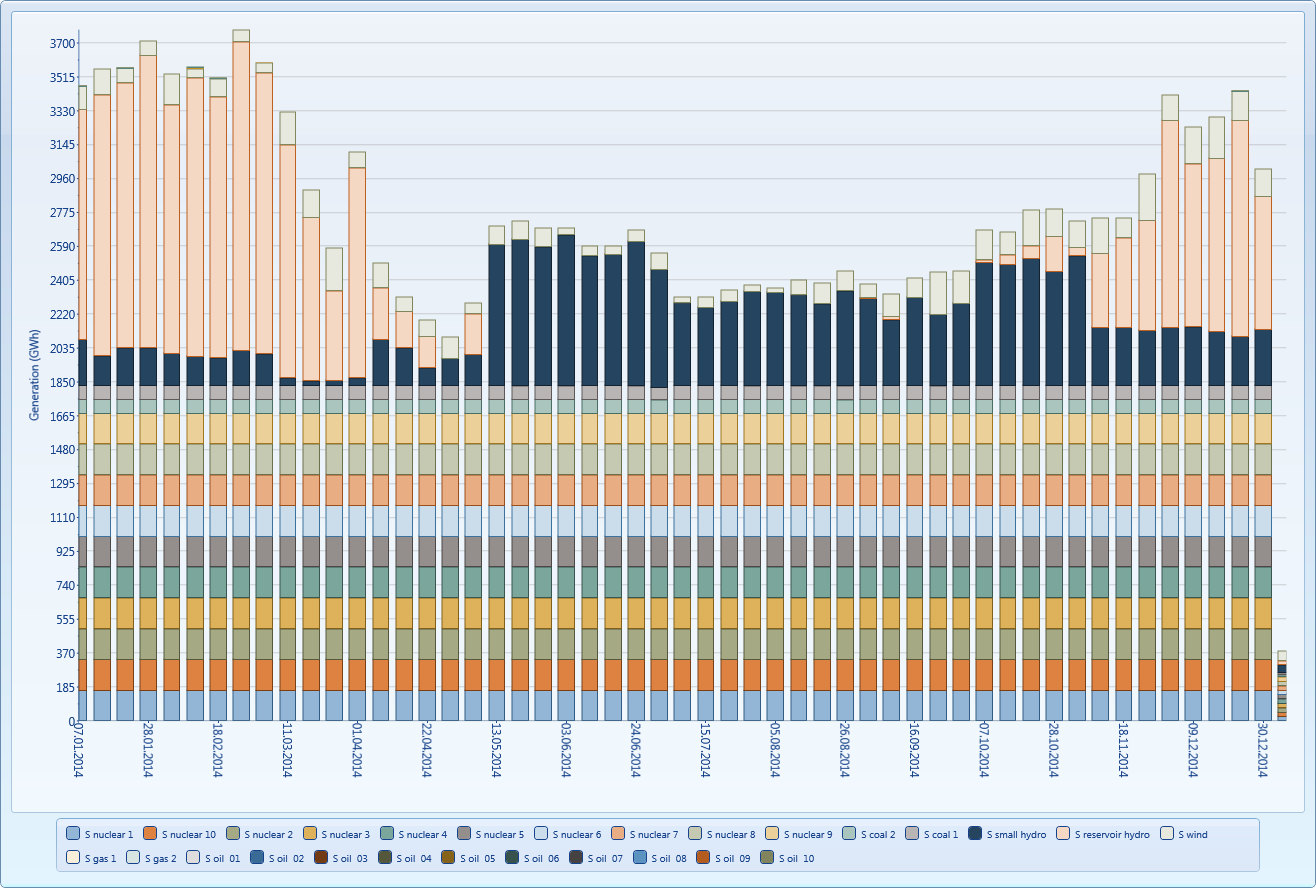
\includegraphics[width=13cm,keepaspectratio=true]{figures/wetcase/MTgenerationSwet}
\caption{Optimal generation dispatch for Sweden 2014 with high inflow}
\label{fig:MTgenerationSwet}
\end{center}
\end{figure}
\begin{figure}[htbp]
\begin{center}
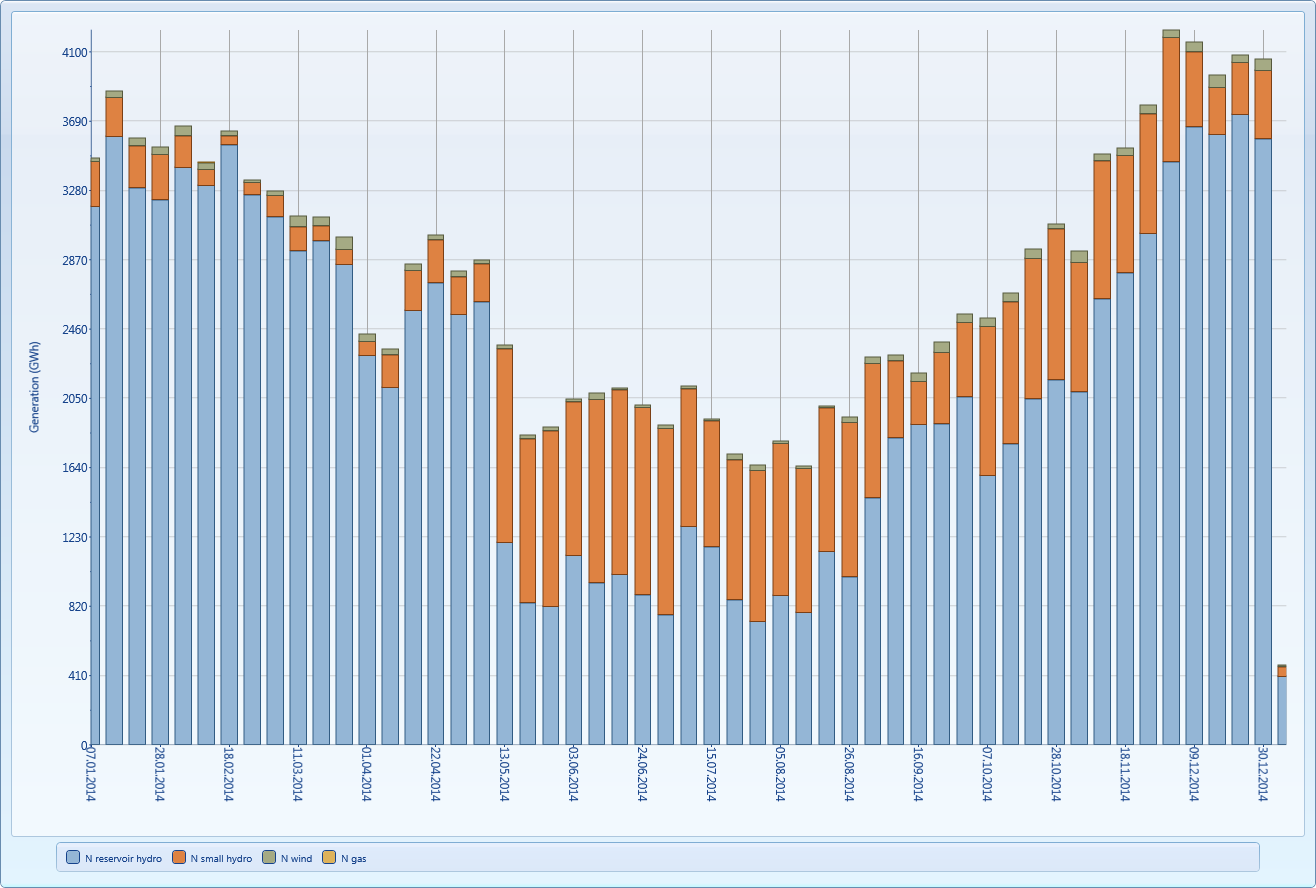
\includegraphics[width=13cm,keepaspectratio=true]{figures/wetcase/MTgenerationNwet}
\caption{Optimal generation dispatch for Norway 2014 with high inflow}
\label{fig:MTgenerationNwet}
\end{center}
\end{figure}
\paragraph{transmission\\}
The usage of the transmission lines between Sweden, Norway and Germany for high inflow into reservoirs is shown in figure \ref{fig:MTnodetransmissionwet}.
\begin{figure}[htbp]
\begin{center}
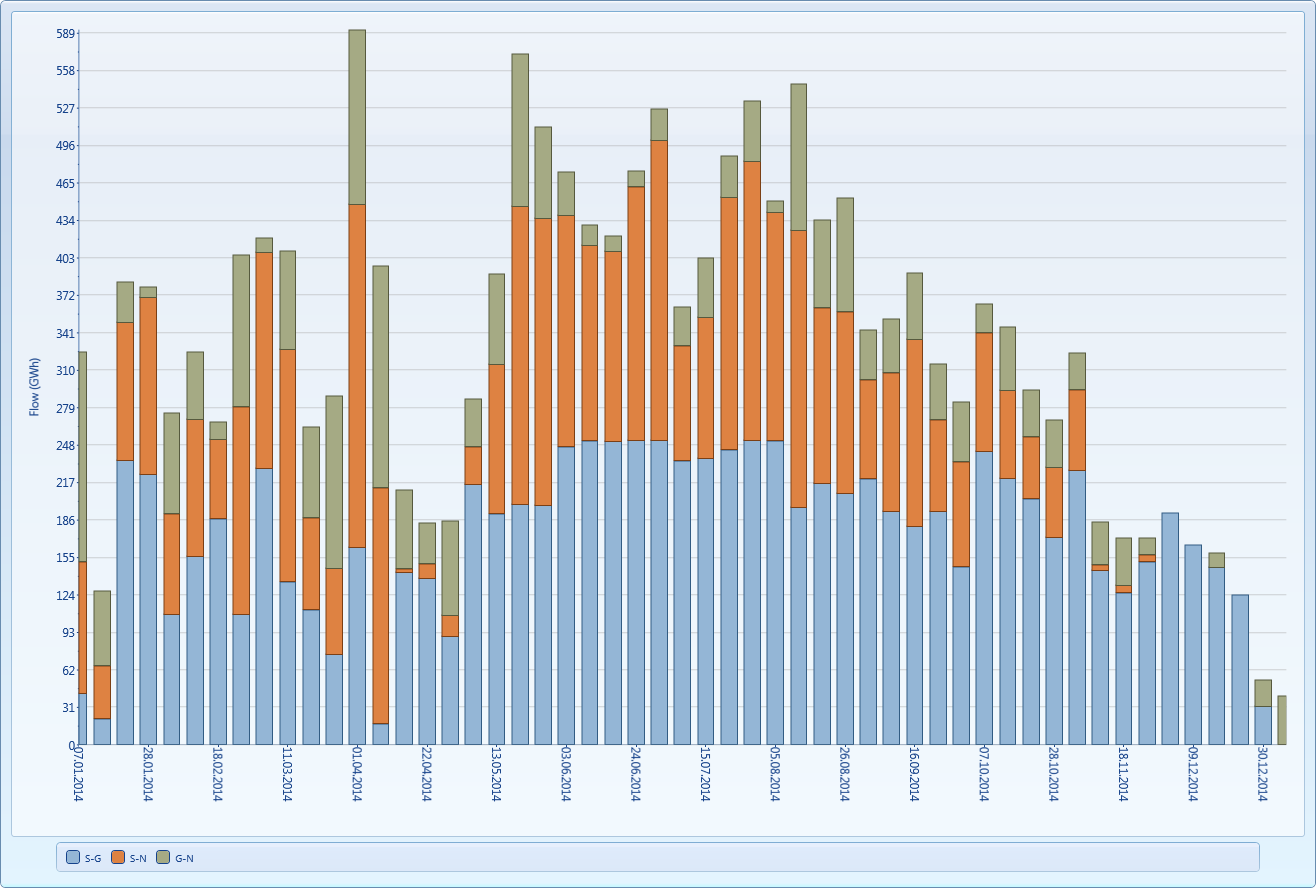
\includegraphics[width=13cm,keepaspectratio=true]{figures/wetcase/MTnodetransmissionwet}
\caption{Transmission between N/W/S with high inflow}
\label{fig:MTnodetransmissionwet}
\end{center}
\end{figure}
\paragraph{emission\\}
Emissions of carbon dioxide by running thermal power plants for this scenario are plotted in figure \ref{fig:MTemissionswet}.
\begin{figure}[htbp]
\begin{center}
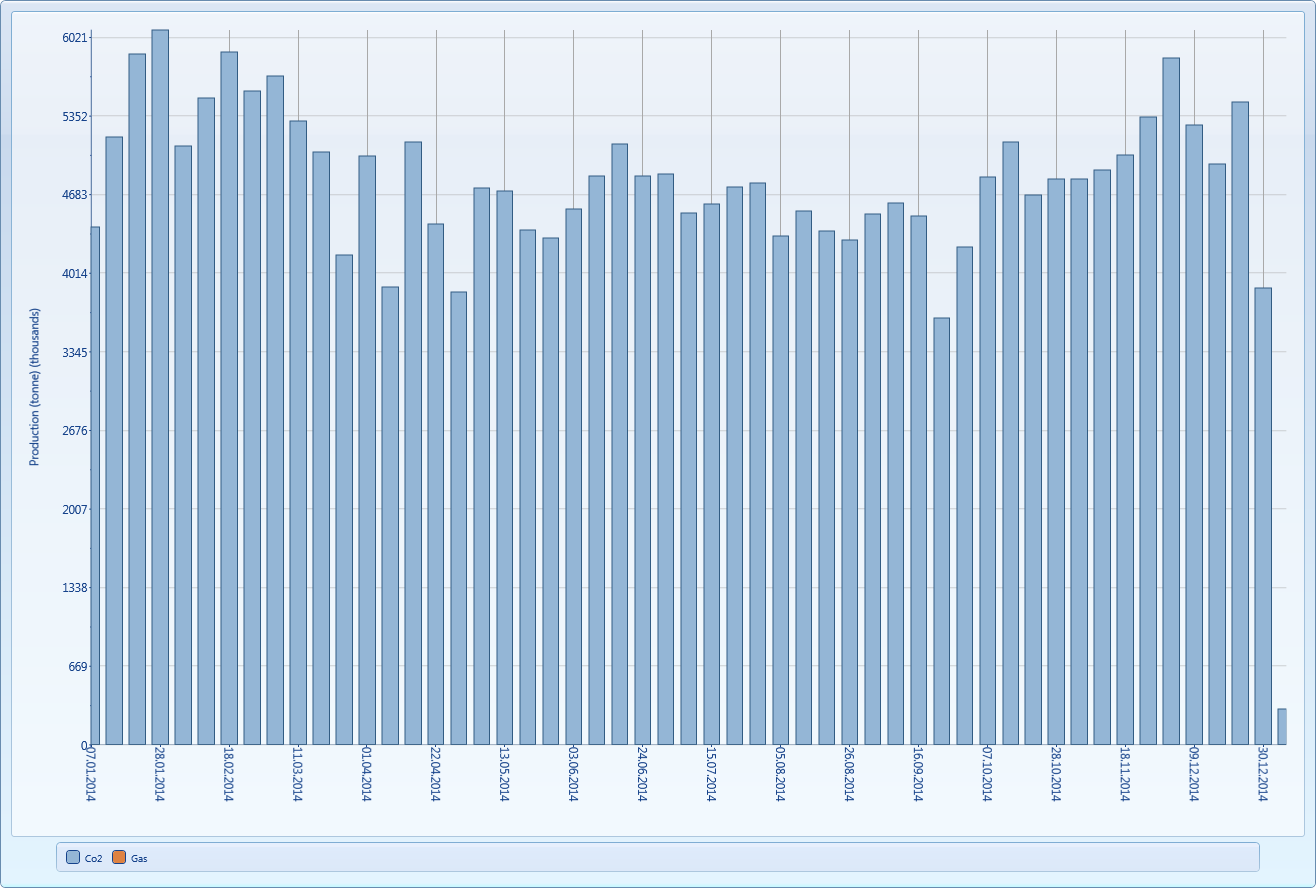
\includegraphics[width=13cm,keepaspectratio=true]{figures/wetcase/MTCO2wet}
\caption{Total $CO_2$-emissions for high inflow 2014}
\label{fig:MTemissionswet}
\end{center}
\end{figure}
\paragraph{price\\}
The energy prices for a whole year 2014 with high inflow is shown in figure \ref{fig:MTpriceswet}.
\begin{figure}[htbp]
\begin{center}
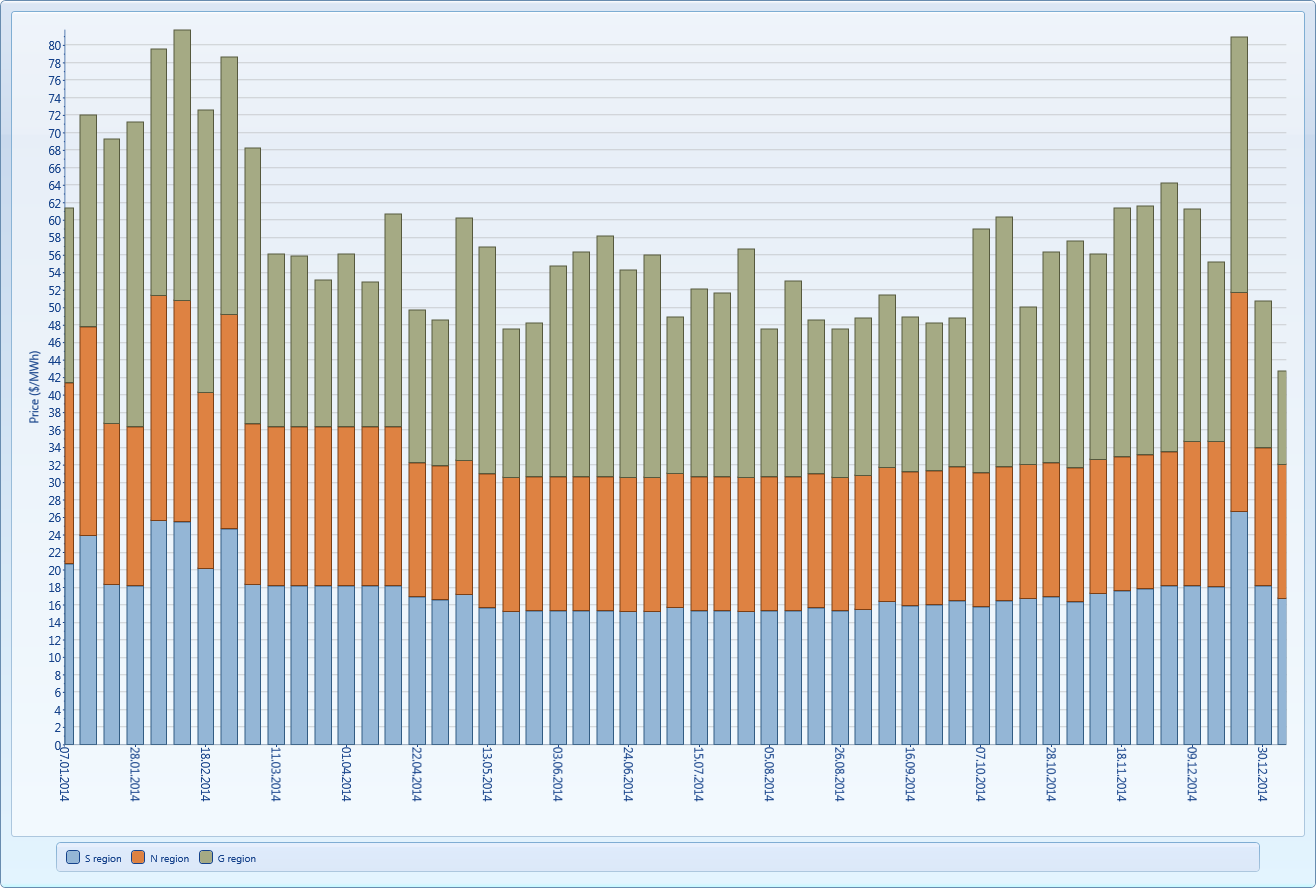
\includegraphics[width=13cm,keepaspectratio=true]{figures/wetcase/MTpriceswet}
\caption{Calculcated prices with high inflow}
\label{fig:MTpriceswet}
\end{center}
\end{figure}

%-------------------------------------------------------------------------------
% expansion planning
%-------------------------------------------------------------------------------
\subsection{Expansion planning}
\newpage
\section{Conclusion}


\end{document}
